\chapter{Question 1}
\label{intro}

\textbf{Determine if the friendship paradox holds for my Facebook account.* Compute the mean, standard deviation, and median of the number of friends that my friends have.  Create a graph of the number of friends (y-axis) and the friends themselves, sorted by number of friends (x-axis).  (The friends don't need to be labeled on the x-axis: just f1, f2, f3, ... fn.)  Do include me in the graph and label me accordingly.\\
$*$ = This used to be more interesting when you could more easily download your friend's friends data from Facebook.  Facebook now requires each friend to approve this operation, effectively making it impossible.\\
I will email to the list the XML file that contains my Facebook friendship graph ca. Oct, 2013.  The interesting part of the file looks like this (for 1 friend):\\}
\begin{verbatim}
<node id="Johan_Bollen_1448621116">
        <data key="Label">Johan Bollen</data>
        <data key="uid"><![CDATA[1448621116]]></data>
        <data key="name"><![CDATA[Johan Bollen]]></data>
        <data key="mutual_friend_count"><![CDATA[37]]></data>
        <data key="friend_count"><![CDATA[420]]></data>
</node>
\end{verbatim}
\textbf{It is in GraphML format: {\url{http://graphml.graphdrawing.org/}}}\\

Following are the steps that I have taken to solve the problem:
\begin{itemize}
\item I downloaded the XML file with the facebook friendship graph and using the `xml.etree' library I parsed through the graph to retrieve the user name and friend count. 
\item I stored the retrieved data in a file `friendNameAndCount'. This code is listed in Listing \ref{lst:q1code1}
\item The sample output of the above mentioned file with user name and friend count is in Figure \ref{fig:q1fig1}
\begin{figure}[h!]
\begin{center}
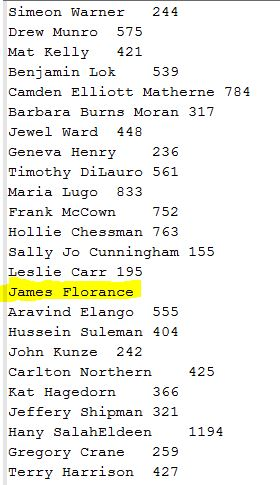
\includegraphics[scale=0.55, keepaspectratio=true]{figures/data.JPG}
\caption{Output file with user name and friend count}
\label{fig:q1fig1}
\end{center}
\end{figure}
\item As highlighted in Figure \ref{fig:q1fig1}, I noticed that 11 friends did not have a friend count. Their names are as follows `James Florance', `Joy Gooden', `Kim Beveridge', `Alfredo Snchez', `Sarah Shreeves', `Sally Mauck', `Dan Swaney', `Robert Gordeaux', `Joseph Kaplan', `Michael Milner' and `Catherine Kemble Cronin'. 
\item I stored only the friend count in a file `friendCount'. By taking this file as input I calculated the mean, median and standard deviation of the number of friends that your friends have. This code is listed in Listing \ref{lst:q1code2}. The output of mean, median and standard deviation are given in Table \ref{Table:q1table1}.

\begin{table}

\caption{Mean, Median and Standard Deviation of number of friends of friends}
\label{Table:q1table1}
\begin{center}
\begin{tabular}{| c | c |}
\hline
Key & Value \\ \hline

Mean & 358.987012987 \\ \hline
Median & 266.5 \\ \hline
Standard Deviation & 370.376887498 \\ \hline

\hline

\end{tabular}
\end{center}
\end{table}

\newpage
\item Figure \ref{fig:q1fig3} illustrates your ranking(in red) in terms of number of friends(y-axis) in comparison to your friends.
\begin{figure}[h!]
\begin{center}
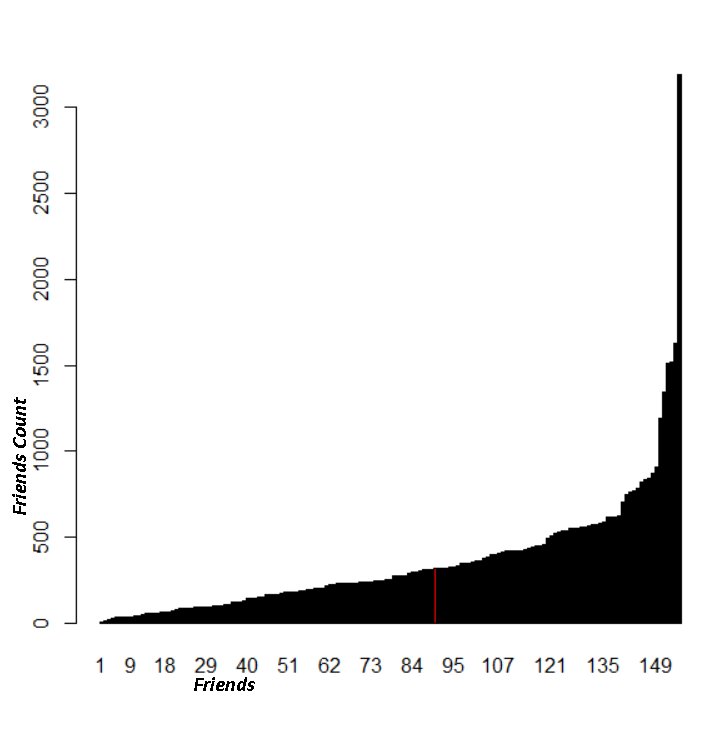
\includegraphics[scale=0.55, keepaspectratio=true]{figures/q1final.PNG}
\caption{Graph with number of friends on y-axis and the friend index on x-axis }
\label{fig:q1fig3}
\end{center}
\end{figure}
\item In conclusion, the above figure clearly indicates that you have less number of friends in comparison to your friends.
\end{itemize}

\newpage
\textbf{Code Listing}
\lstset{tabsize = 2}
\lstinputlisting[language=Python,caption=Python code for extracting friends count from XML file,frame=single,breaklines=true,label=lst:q1code1,captionpos=b,numbers=left,showspaces=false,showstringspaces=false,basicstyle=\footnotesize]{src/getFriendsCount.py}

\newpage
\textbf{Code Listing}
\lstinputlisting[language=Python,caption=Python code for calculating mean median and standard deviation,frame=single,breaklines=true,label=lst:q1code2,captionpos=b,numbers=left,showspaces=false,showstringspaces=false,basicstyle=\footnotesize]{src/getMeanMedianStandardDeviation.py}